\section{Preliminaries}
\label{sec:l2cpcc}
In this section, we first provide a background of structured representation learning and then discuss the limited representation capacity of the Euclidean space for hierarchical information, which serves as the primary motivation for our work. 

\subsection{Background}

Structured representation learning \citep{zeng2022learning} breaks the permutation invariance of flat representation learning by incorporating a hierarchical regularization term with a standard classification loss. The regularization term is specifically designed to enforce class-conditioned grouping or partitioning in the feature space, based on a given hierarchy.

More specifically, given a weighted tree $\mathcal{T} = (V, E, e)$ with vertices $V$, edges $E$ and edge weights $e$, let us compute a tree metric $d_\mathcal{T}$ for any pair of nodes $v,v' \in V$, as the weighted length of the shortest path in $\mathcal{T}$ between $v$ and $v'$. For a real world dataset $\data = \{(\vx_i, y_i)\}_{i = 1}^N$, we can specify a \emph{label tree} $\mathcal{T}$ where a node $v_i\in V$,  $v_i$ corresponds to a subset of classes, and $\data_i\subseteq \data$ denote the subset of data points with class label $v_i$. We denote dataset distance between $\data_i$ and $\data_j$ as $\rho(v_i, v_j) = d\left(\data_i,\data_j\right)$, where $d(\cdot, \cdot)$ is any distance metric in the feature space, varied by design.

With a collection of tree metric $d_\mathcal{T}$ and dataset distances $\rho$, we can use the Cophenetic Correlation Coefficient (CPCC) \citep{cpcc}, inherently a Pearson's correlation coefficient, to evaluate the correspondence between the nodes of the tree, and the features in the representation space. Let $\overline{d_\mathcal{T}}, \overline{\rho}$ denote the mean of the collection of distances, then CPCC is defined as
\begin{equation}
\label{eq:CPCC}
    \cpcc(d_\mathcal{T}, \rho) := \frac{\sum_{i<j}(d_\mathcal{T}(v_i,v_j) - \overline{d_\mathcal{T}})(\rho(v_i,v_j) - \overline{\rho})}{(\sum_{i<j}(d_\mathcal{T}(v_i,v_j) - \overline{d_\mathcal{T}})^2)^{1/2} (\sum_{i<j}(\rho(v_i,v_j) - \overline{\rho})^2)^{1/2}}. 
\end{equation}
For the supervised classification task, we consider the training set  $\mathcal{D}_{\text{tr}}^{\text{in}} = \{(\vx_i, y_i)\}_{i=1}^N$ and we aim to learn the network parameter $\theta$ for a feature encoder $f_\theta : \mathcal{X} \to \gZ$, where $\gZ \subseteq \mathbb{R}^{d}$ denotes the representation/feature space. For structured representation learning, the feature encoder is usually followed by a classifier $g_{w}$, and the parameters $\theta, w$ are learnt by minimizing $\gL$ along with a standard \emph{flat} (non-hierarchical) classification loss, for instance, Cross-Entropy (\texttt{CE}) or Supervised Contrastive (\texttt{SupCon}) \citep{2020supcon} loss, with the structured regularization term as:
\begin{equation}
    \label{eq:objective_regularizer}
    \mathcal{L}(\data) = \sum_{(\vx, y)\in \data} \ell_\text{Flat}(\vx,y,\theta, w) - \alpha\cdot\cpcc(\tmetric, \rho).        
\end{equation}
Using a composite objective as defined in~\Cref{eq:objective_regularizer}, we can enforce the distance relationship between a pair of representations in the feature space, to behave similarly to the tree metric between the same vertices. For instance, consider a simple label tree with a root node, a coarse level, and a fine level, where subsets of fine classes share the same coarse parent. For this hierarchy, we would expect the fine classes of the same parents (e.g., \emph{apple} and \emph{banana} are \emph{fruits}) to have closer representations in the feature space, whereas fine classes with different coarse parents (e.g., an \emph{apple} is a \emph{fruit} and a \emph{tulip} is a \emph{flower}) should be further apart. The learned structure-informed representations reflect these hierarchical relationships and lead to interpretable features with better generalization \citep{zeng2022learning}.

\subsection{$\ell_2$-CPCC}

\Cref{eq:CPCC} offers the flexibility of designing a metric to measure the similarity between two data subsets, and \citet{zeng2022learning} define the \emph{Euclidean dataset distance} as $\rho_{\ell_2}(\data_i, \data_j) := \|\frac{1}{|\data_i|}\sum_{\vx\in \data_i}f(\vx) - \frac{1}{|\data_j|}\sum_{\vx'\in \data_j}f(\vx')\|_2$. The distance between datasets is thus the $\ell_2$ distance between two Euclidean \emph{centroids} of their class-conditioned representations, which is unsuitable for modeling \emph{tree-like} data \citep{chen2013hyperbolicity}. 
Additionally, this regularization approach in \citet{zeng2022learning} is applied only to the leaf nodes of $\mathcal{T}$ for efficiency.

However, this leaf-only formulation of the CPCC offers an \emph{approximation} of the structured information, since the distance between non-leaf nodes is not restricted explicitly by the regularization. This approximation, therefore, leads to a loss of information contained in the original hierarchy $\mathcal{T}$.

Actually, it is impossible to embed $d_\mathcal{T}$ into $\ell_2$ exactly. Or more formally, there exists no bijection $\varphi$ such that $d_\mathcal{T}(\varphi(\vz_i), \varphi(\vz_j)) = \lVert \vz_i - \vz_j \rVert_2$ irrespective of how large the feature dimension $d$ is. We provide two such examples for a toy label tree in \Cref{fig:failure}, below. 

\begin{wrapfigure}{l}{0.4\textwidth}
\centering
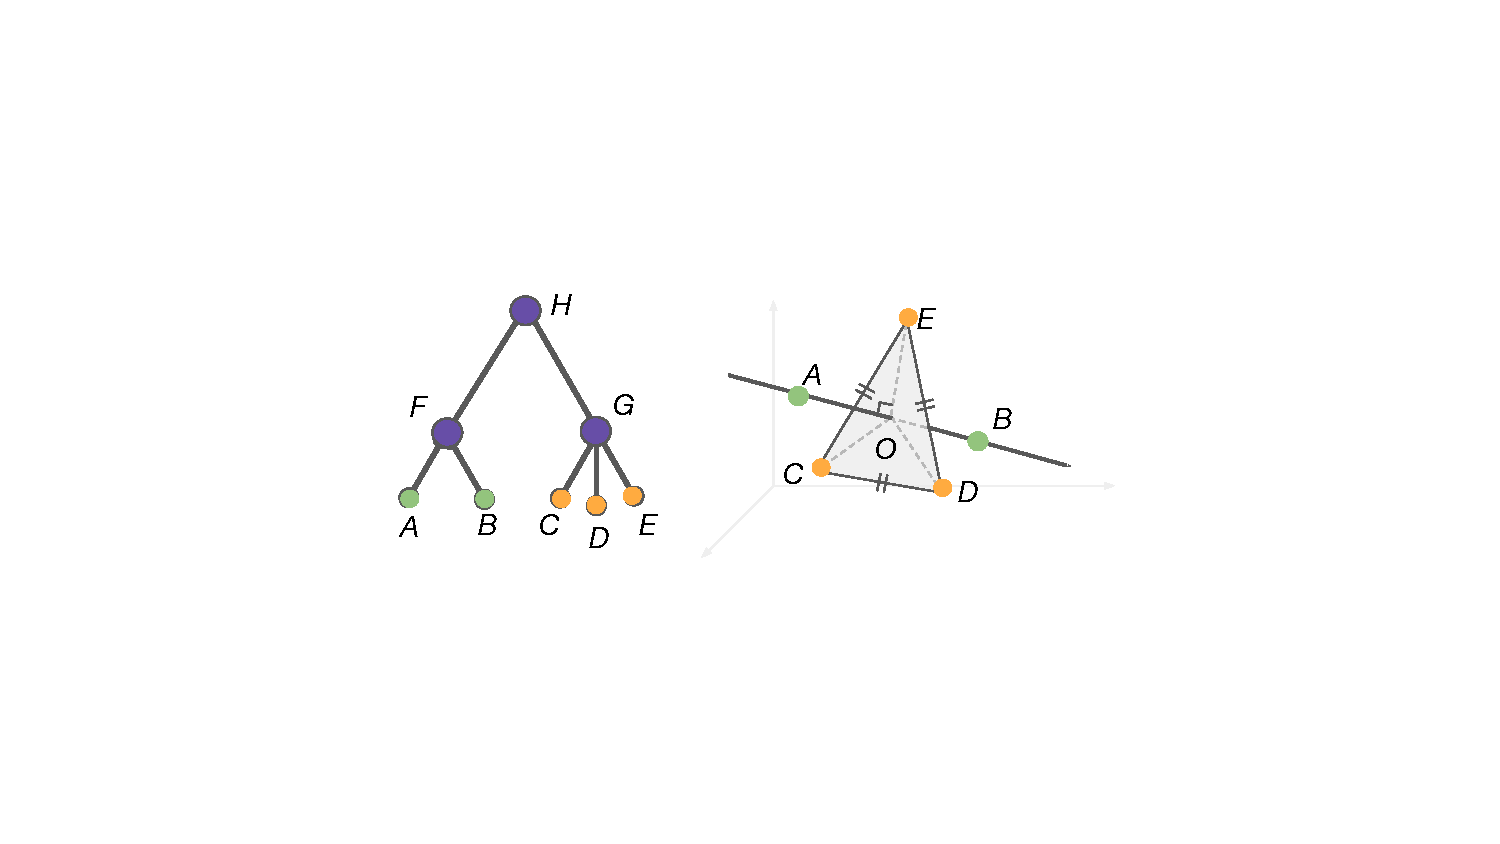
\includegraphics[width=\linewidth]{figures/l2_failure.pdf}\hspace*{-0.4cm}
\caption{(left) An unweighted label tree with two coarse nodes: $F$, $G$. $F$ contains two fine classes $A,B$ and $G$ contains three fine classes $C,D,E$. We cannot embed this in $\ell_2$ exactly (right).}
\vspace{-1em}
\label{fig:failure}
\end{wrapfigure}

\textbf{Example 1.} We intend to embed all nodes in $\gT$, including purple internal nodes. Notice that $G,C,D,E$ is a star graph centered at $G$. Since $CG = DG = 1, CD = 2$, by triangle inequality $C,D,G$ must be on the same line where $G$ is the center of $CD$. Similarly, $G$ must be at the center of $DE$. Hence, the location of $E$ must be at $C$, which contradicts the uniqueness of all nodes in $\gT$.

\textbf{Example 2.} As an easier problem, let us only embed leaf nodes into the Euclidean space as shown in \Cref{fig:failure}. Since $CD = DE = CE = 2$, they must be on a plane with an equilateral triangle $\triangle_{CDE}$ in Euclidean geometry. Then all the green classes have the same distance $4$ to each yellow class. Therefore, $A,B$ must be on the line perpendicular to $\triangle_{CDE}$ and intersecting the plane with $O$, which is the barycenter of $\triangle_{CDE}$. Due to the uniqueness and symmetry of $A,B$, we must have $AO = BO = 1$ to satisfy $AB = 2$. $AO = 1, OE = \frac{2\sqrt{3}}{3}, AE = 4$ which contradicts the Pythagorean Theorem.

\begin{figure}[t]
\vspace{-1em}
\centering
\begin{subfigure}{.5\textwidth}
  \centering
  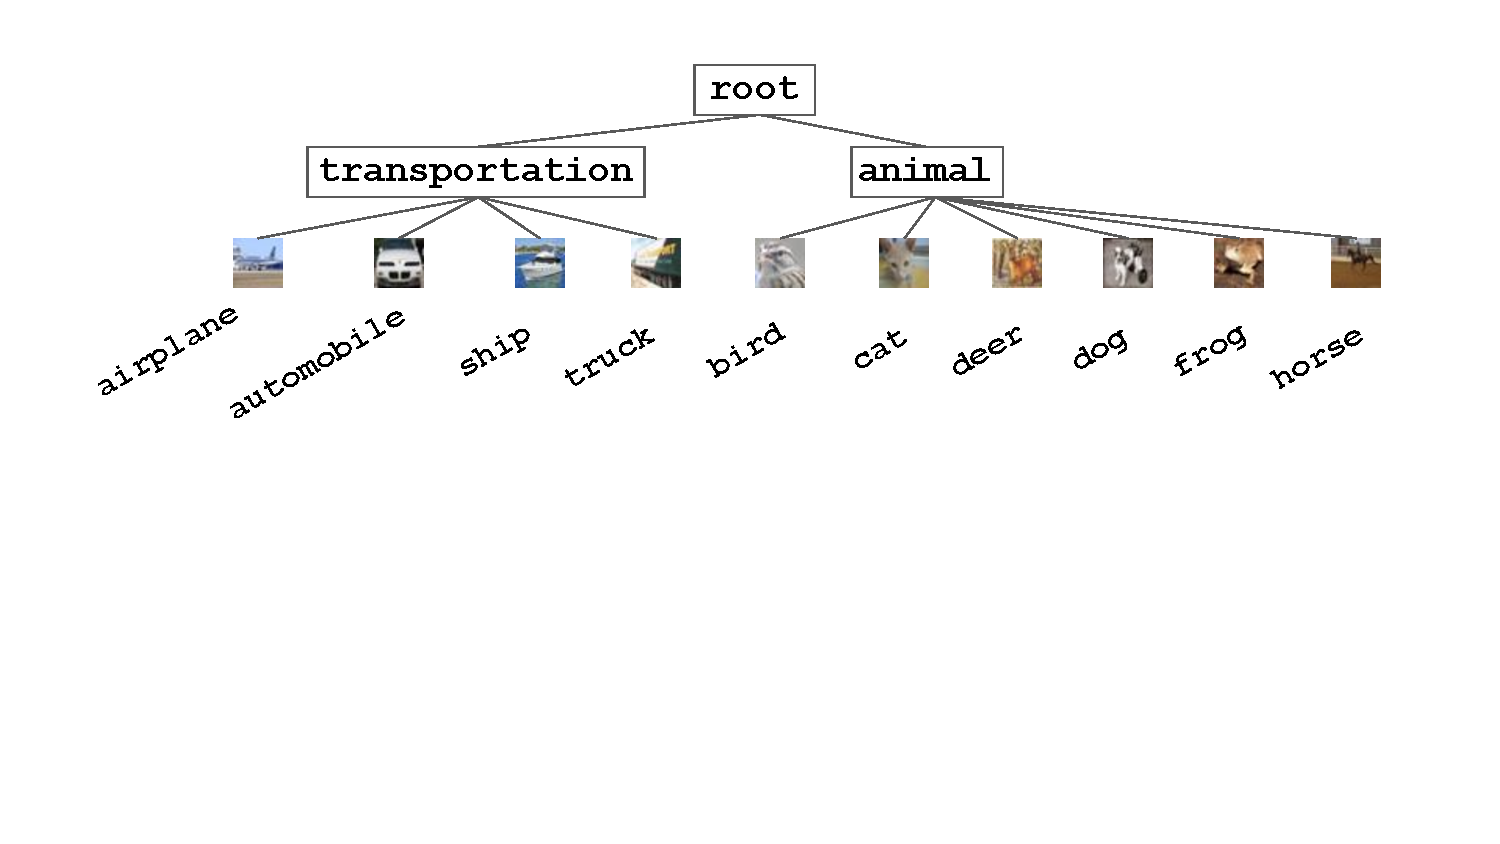
\includegraphics[width=\linewidth]{figures/CIFAR10Tree.pdf}
\end{subfigure}%
\begin{subfigure}{.5\textwidth}
  \centering
  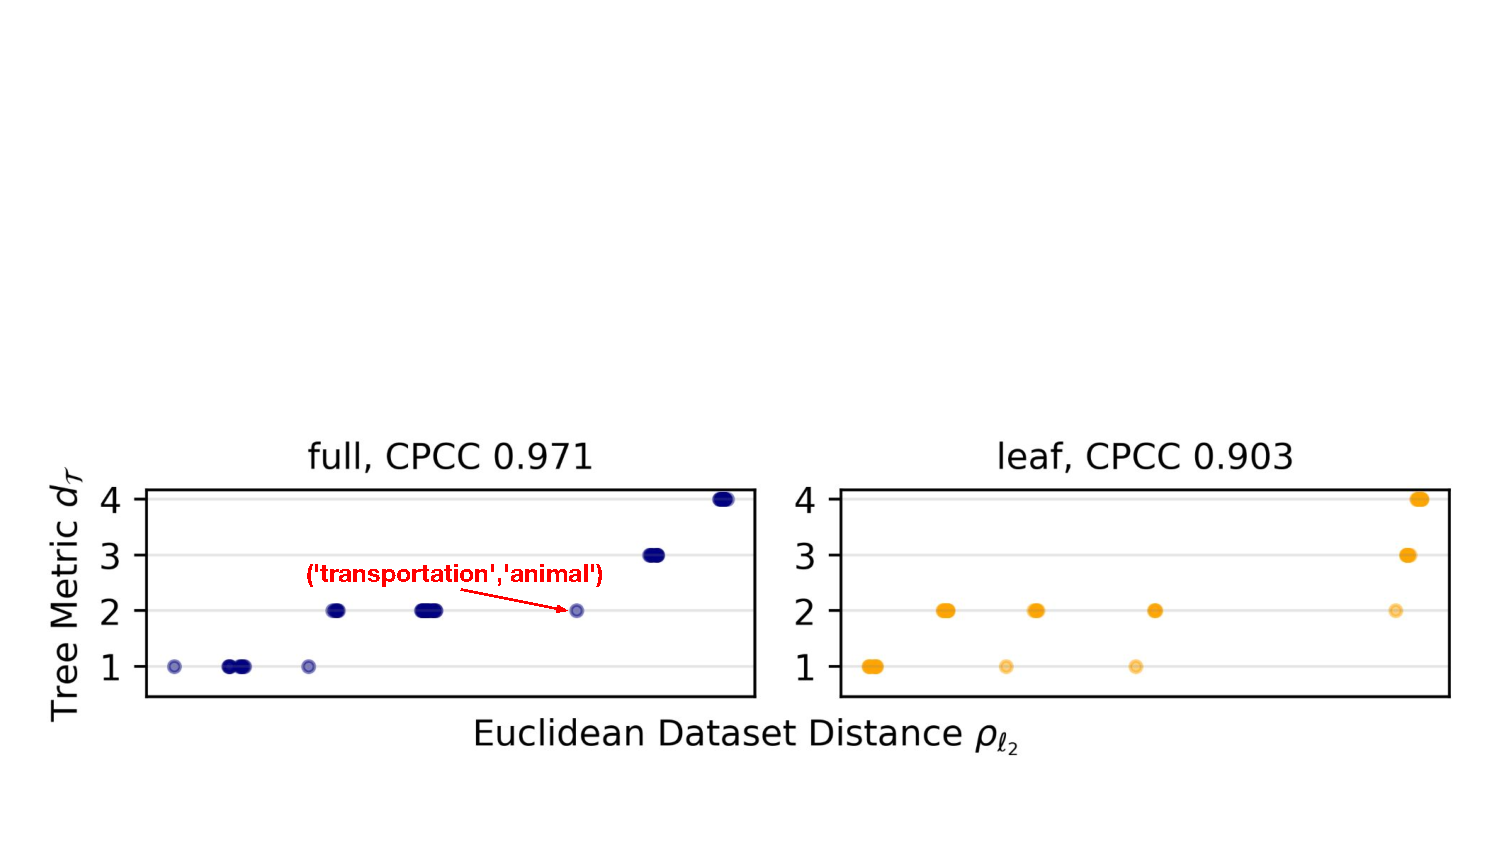
\includegraphics[width=\linewidth]{figures/CIFAR10CPCC.pdf}
\end{subfigure}
\caption{Using $\ell_2$-CPCC for structured representation on CIFAR10. CIFAR10 hierarchy (left) has a three level structure with $13$ vertices. For a $512$-dimensional embedding, we apply $\ell_2$-CPCC either for the full tree (middle) or the leaf nodes only (right) and plot the ground truth tree metric against pairwise Euclidean centroid distances of the learnt representation. The optimal train CPCC is $1$.}
\vspace{-1em}
\label{fig:toy}
\end{figure}

Since we cannot embed an arbitrary tree $\gT$ into $\ell_2$ without distortion, it would also affect the optimization of the $\ell_2$-CPCC in a classification problem, where the tree weights encode knowledge of class similarity. To verify our claims, we consider the optimization of $512$-dimensional $\ell_2$-CPCC structured representations for CIFAR10 \citep{krizhevsky2009learning}. The CIFAR10 dataset consists of a small label hierarchy as shown in \Cref{fig:toy} (left). 

The optimal CPCC is achieved when each tree metric value corresponds to a single $\rho_{\ell_2}$. However, in \Cref{fig:toy} (right), even with an optimization of the $\ell_2$-CPCC loss for the entire tree, we observe a sub-optimal train CPCC less than $1$, where the distance between two coarse nodes, \emph{transportation} and \emph{animal}, is far away from the desired solution. Furthermore, optimization of the CPCC loss for only the leaf nodes, leads to an even larger distortion of the tree metrics. 

